\documentclass{standalone}
\usepackage{tikz}
\usepackage{ctex,siunitx,upgreek}
\setCJKmainfont{Noto Serif CJK SC}
\usepackage{tkz-euclide}
\usepackage{amsmath,amsfonts,amssymb}
\usetikzlibrary{patterns, calc,3d}
\usetikzlibrary {decorations.pathmorphing,decorations.pathreplacing,decorations.shapes}
\tikzset{label style/.append style={font=\small}}
\begin{document}
\small
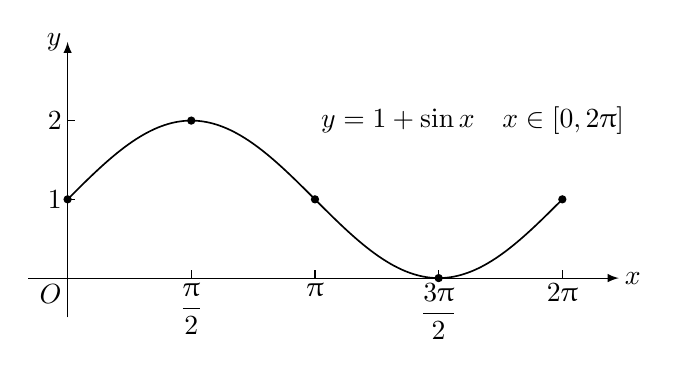
\begin{tikzpicture}[>=latex,scale=1.0,inner sep=2pt]
  \draw[->](-0.5,0)--(7,0)node[right]{$x$};
  \draw[->](0,-0.5)--(0,3)node[left]{$y$};
  \node at (0,0)[below left]{$O$};
  \draw[semithick,samples=200,domain=0:2*pi]plot(\x,{1+sin(\x r)});
  \foreach \x in {1,2}
    {\draw[very thin](0,\x)node[left]{$\x$}--++(0.1,0);}
  \foreach \x[count=\i] in {\dfrac\uppi2,\uppi,\dfrac{3\uppi}{2},2\uppi}
  {
    \fill(\i*pi/2,{1+sin(\i*90)})circle(1.5pt);
    \draw(\i*pi/2,0)node[below]{$\x$}--++(0,0.1);
  }
  \fill(0,1)circle(1.5pt);
  \node at (pi,2)[right]{$y=1+\sin x\quad x\in[0,2\uppi]$};
\end{tikzpicture}
\end{document}